\section{Finite-Delay Ramsey Spectrum and Coherence Linewidth}
\label{sec:ramsey-fft-linewidth}

We compare the echo linewidth with an ideal Ramsey delay scan at the same
coherence time. For short, calibrated $\pi/2$ pulses and exponential free
induction decay, the measured population has the form~\cite{PhysRev.78.695}
\begin{equation}
 P(t)=B+A e^{-t/T_2^*}\cos(2\pi f_Rt+\phi),\qquad 0\leq t<T.
 \label{eq:ramsey-decaying-cosine}
\end{equation}
Here $T$ is the maximum free-evolution delay, $f_R$ is the Ramsey fringe
frequency, and $B$, $A$, and $\phi$ describe the offset, contrast, and phase.
We use the paper's common reference $T_2^*=\PaperTTwoStar~\mu\mathrm{s}$,
not the Hahn-echo coherence time. Figure~\ref{fig:ramsey-fft-linewidth}
uses a noiseless, baseline-subtracted cosine with $f_R=1~\mathrm{MHz}$ and
$\phi=0$; it is a calculated reference, not an additional Ramsey measurement.

\subsection{Finite record and choice of spectrum}

Writing $a=1/T_2^*$, the transform of one isolated frequency component is
\begin{equation}
 G_T(\nu)=\int_0^T e^{-at}e^{-i2\pi\nu t}\,dt
 =\frac{1-e^{-(a+i2\pi\nu)T}}{a+i2\pi\nu}.
 \label{eq:ramsey-finite-transform}
\end{equation}
The real cosine has both positive- and negative-frequency components:
\begin{equation}
 \widetilde{P-B}(f)=\frac{A}{2}
 \left[e^{i\phi}G_T(f-f_R)+e^{-i\phi}G_T(f+f_R)\right].
 \label{eq:ramsey-cosine-transform}
\end{equation}
For well-separated components, the line near $f_R$ is described by $G_T$.
In the long-record limit, with $x=2\pi\nu T_2^*$,
\begin{align}
 \frac{\operatorname{Re}G_\infty(\nu)}{G_\infty(0)}
 &=\frac{|G_\infty(\nu)|^2}{|G_\infty(0)|^2}
 =\frac{1}{1+x^2},\\
 \frac{|G_\infty(\nu)|}{G_\infty(0)}&=\frac{1}{\sqrt{1+x^2}}.
\end{align}
Consequently, the phase-corrected real (absorptive) spectrum and the power
spectrum have FWHM $\Gamma_{T_2^*}=1/(\pi T_2^*)=41.88~\mathrm{kHz}$.
The magnitude spectrum, often plotted as \texttt{abs(FFT)}, instead has
FWHM $\sqrt{3}\,\Gamma_{T_2^*}=72.54~\mathrm{kHz}$ even for an infinitely
long record. These conventions must be distinguished before comparing
linewidths. Their finite-$T$ widths also differ, as shown in
Table~\ref{tab:ramsey-fft-linewidth}.

\begin{table}[tb]
 \caption{Calculated Ramsey FWHM in kHz for $T_2^*=7.6~\mu\mathrm{s}$.
 Widths are the separation of the first half-height crossings of the
 isolated central line in Eq.~\eqref{eq:ramsey-finite-transform}, with a
 rectangular delay window and no additional filtering.}
 \label{tab:ramsey-fft-linewidth}
 \centering
 % Generated by scripts/make_supplemental_ramsey_fft.py
\begin{tabular}{rccc}
\hline\hline
$T$ ($\mu\mathrm{s}$) & $\operatorname{Re}G_T$ & $|G_T|^2$ & $|G_T|$ \\
\hline
5 & 133.43 & 179.53 & 245.37 \\
10 & 74.69 & 93.32 & 128.91 \\
20 & 48.28 & 53.93 & 78.57 \\
30 & 42.59 & 44.35 & 72.86 \\
40 & 41.80 & 42.08 & 73.54 \\
$\infty$ & 41.88 & 41.88 & 72.54 \\
\hline\hline
\end{tabular}

\end{table}

\subsection{Delay range, sampling, and analysis}

At $T=20~\mu\mathrm{s}=2.63T_2^*$, the absorptive linewidth is
$48.28~\mathrm{kHz}=1.153\Gamma_{T_2^*}$; the power-spectrum width is
$53.93~\mathrm{kHz}=1.288\Gamma_{T_2^*}$. Extending the scan to
$40~\mu\mathrm{s}=5.26T_2^*$ gives 41.80 and $42.08~\mathrm{kHz}$,
respectively, both within 1\% of the infinite-record value. A delay span
of approximately five to six decay times is therefore sufficient here
to display a nearly coherence-limited Fourier line. Rectangular-window
ripples cause a small, nonmonotonic approach to the limiting width.

For an experimental analysis, fit Eq.~\eqref{eq:ramsey-decaying-cosine}
with $B$, $A$, $\phi$, $f_R$, and $T_2^*$ free, and subtract the fitted
offset before transforming. Phase-correct the positive-frequency component
to report its absorptive linewidth, or explicitly report a power-spectrum
linewidth. A direct time-domain fit gives the intrinsic model linewidth
$1/(\pi T_{2,\mathrm{fit}}^*)$ without interpreting finite-window broadening
as faster decay; the precision of that inference still depends on noise
and the measured delay range. If the decay is not exponential, the
Lorentzian relation must be replaced by the appropriate line shape.

Uniform delay sampling must resolve the largest fringe frequency in the
search range. For the illustrated $1~\mathrm{MHz}$ fringes, a step of
$50~\mathrm{ns}$ gives 20 samples per period; the numerical FFT uses
$10~\mathrm{ns}$ to reduce discretization error. Its complex spectrum
agrees with Eq.~\eqref{eq:ramsey-cosine-transform} to within 0.2\% of
the peak amplitude over the displayed window. The unpadded FFT spacing
is $1/T$, or $50~\mathrm{kHz}$ for a $20~\mu\mathrm{s}$ scan.
Zero padding interpolates the spectrum to locate half-height crossings;
it adds no measurement information. Extra apodization changes the
linewidth and must be included in the model if used.

\subsection{Comparison with the shaped echo}

The $20~\mu\mathrm{s}$ polynomial-corrected DRAG echo in Fig.~3 of the
Letter has a measured median FWHM of approximately
$\LatestPolyWidthNormalized\Gamma_{T_2^*}$ on the common accepted amplitudes.
Ideal Ramsey is narrower at the same maximum evolution time: its
$20~\mu\mathrm{s}$ absorptive width is only $1.15\Gamma_{T_2^*}$, and even
the magnitude width is $1.88\Gamma_{T_2^*}$. Thus the echo's
approximately three-to-four-reference linewidth is not a linewidth
advantage over ideal Ramsey. Its demonstrated property is a resolved
frequency-swept response over a broad drive-amplitude range. A Ramsey
delay scan and an echo frequency scan both require repeated preparation
and readout at many settings; equal maximum evolution time does not
imply equal total acquisition time or frequency-estimation uncertainty.

\begin{figure*}[!tp]
 \centering
 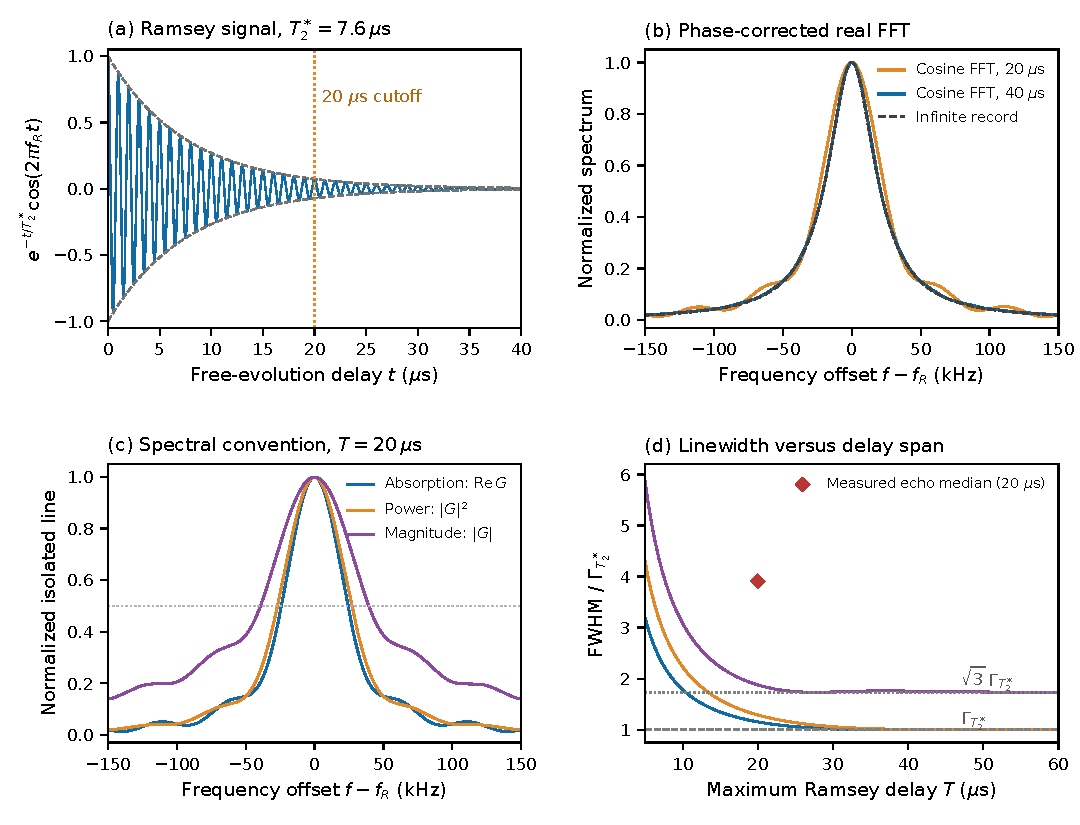
\includegraphics[width=\textwidth]{supplemental/ramsey_fft_linewidth.pdf}
 \caption{Ramsey Fourier-line reference for $T_2^*=7.6~\mu\mathrm{s}$.
 (a) Exponentially damped cosine at $f_R=1~\mathrm{MHz}$; dashed curves
 give its envelope and the vertical line marks a $20~\mu\mathrm{s}$ cutoff.
 (b) Real FFTs of the actual cosine sampled over 20 and $40~\mu\mathrm{s}$,
 compared with the infinite-record isolated absorptive line. The known
 phase and baseline are zero. (c) Absorption, power, and magnitude
 conventions for the isolated $20~\mu\mathrm{s}$ line.
 (d) Their FWHM versus maximum Ramsey delay; colors match (c).
 The red diamond is the measured corrected-echo median from Fig.~3,
 included as a linewidth reference rather than a measurement-time benchmark.
 All spectra are normalized to their own peak. FFTs use a $10~\mathrm{ns}$
 step and $2^{18}$ points after zero padding, with no apodization;
 linewidth curves use the exact finite-record transform.}
 \label{fig:ramsey-fft-linewidth}
\end{figure*}
